\documentclass[11pt]{article}

\usepackage{array}
\usepackage{graphicx}
\usepackage[letterpaper]{geometry}

\title{Measuring the Complexity of All the Art}
\author{Jonathan Langke and Peter Boothe}
\date{\today}

\begin{document}
\maketitle

\begin{abstract}
We have measured (using Racket and MiniKanren) the Kolmogorov Complexity of all
possible 2x2 and 3x2 artworks.  We have also conducted a survey of the relative
perceived visual complexity of these artworks.  In this paper, we discuss both
our generation strategy as well as the results of our online survey.
\end{abstract}

\section{Introduction}

Art has many definitions, but the one we will use here is that a piece of black
and white digital art is a matrix where every entry is either true or false.
An artwork can be generated from a mathematical formula that evalutes to a
boolean and involves integers $x$ and $y$.  For our initial study, we
considered only 2x2 matrices, because there are only $2^{2\cdot2} = 16$ of
them, and they could therefore be exhaustively generated.

The Kolmogorov Complexity or program-size complexity of a particular object is
the size of the smallest program which outputs that object.  This allows us to
talk about the complexity (and randomness) of individual items.  Kolmogorov
complexity is, unfortunately, uncomputable.  It is, however, recursively
enumerable (RE).  Therefore, we can enumerate all well-typed expressions and
evaluate them on multiple inputs.  The size of the smallest expression which
outputs that object is then its Kolmogorov complexity!

Our algorithm to generate all the art, and keep track of its Kolmogorov
Complexity is as follows: Enumerate all well-typed programs of size 1.  For
each enumerated formula, generate its corresponding artwork.  If this artwork
has not been previously generated, then it has Kolmogorov complexity 1.  Next,
we repeat for size 2, 3, 4, etc., until we have managed to generate all
possible 2x2 artworks.  To do this, however, we must first define what we mean
by a ``well-typed program''.

A program is well-typed if the inputs types of the functions match the type of those function's arguments.  An example of an ill-typed program is {\tt (+ false 3)}, whereas a well-typed program is {\tt (+ 3 x)}.  We further require that the overall type of our program be {\tt (int, int) -> bool}.  An example of such an expression is {\tt ($\lambda$ (x y) (< x y))}, which is an expression with two inputs, which evalutes to either true or false.

Further, we also need to define our programming language.  Our language is constructed out of the atoms {\tt < + * x y 1 0 and or not true false}.  With this description, we use MiniKanren, a logic programming system for Racket, to generate a list of all well-typed programs in order of size.

\subsection{Racket/MiniKanren}

To fully understand the power of Racket and MiniKanren one needs to understand 
how it is that Logic Languages operate. MiniKanren (like any logic language) is
used to satisfy relationships specified by the user. In our application this was used
to generate all formulae up to a particular size(in symbols) and then produce the
corresponding pictorial output (depicted below). 

% Need to move PNGs here I think but other than that good segway into concretizing
% The concept

\subsection{Example}
\begin{figure}
\begin{center}
\begin{tabular}{r | p{2in}   p{2in}}
Expression & (x $<$ y) &
(((1 + (1 + 1)) $<$  (x * y)) and 
          ((x + 1) $<$ (y * (1 + 1)))) \\
Expression Size & 3 symbols & 19 symbols\\
  Artwork & 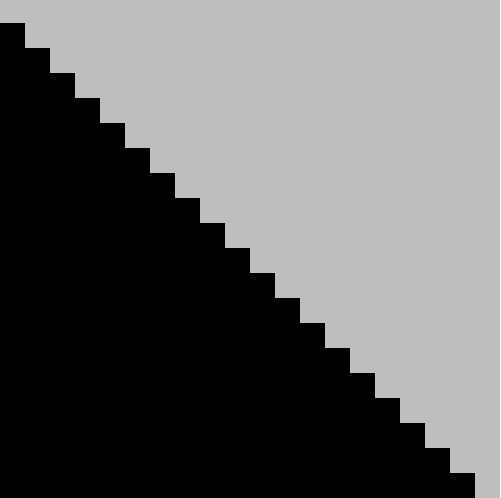
\includegraphics[width=1.5in]{../presentation/simple.png} &
  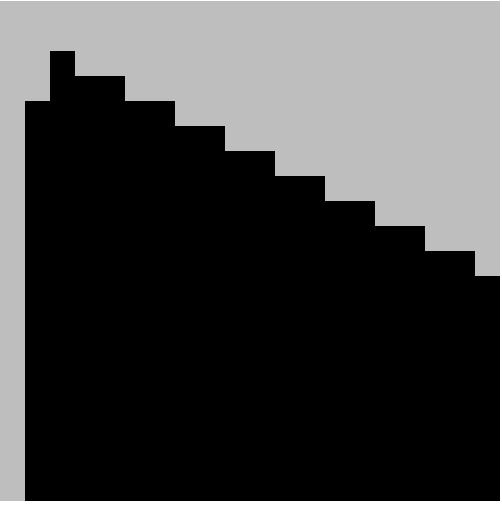
\includegraphics[width=1.5in]{../presentation/complex.png} \\
Kolmogorov Complexity& 3 &
19
\end{tabular}
\end{center}

\caption{Two artworks of differing Kolmogorov Complexity}
\end{figure}


\section{Generating The Art}

After generating all the formulae to a particular size the next step in our algorithm is
to generate all the art corresponding to each formulae as depicted in the example seen
previously. When we where able to produce all the 2x2 art we where able to garner a lot of
insight into the interrelatedness of the different artwork.

\subsection{All the 2x2 Art}
\begin{figure}
\begin{center}
\begin{tabular}{r c l}
Formulae & Level & Pictures \\
\tiny{none} & 0 & empty \\
\tiny{(true), (false)} & 1 &
    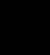
\includegraphics[width=.25in]{../presentation/2x2/Shape1LVL1.png}~
    
\includegraphics[width=.25in]{../presentation/2x2/Shape2LVL1.png} \\
\tiny{none} & 2 & empty \\
\tiny{($<$ x 1), ($<$ y 1), ($<$ x y), ($<$ 0 x), ($<$ 0 y), ($<$ y x)} & 3 & 
    
\includegraphics[width=.25in]{../presentation/2x2/Shape1LVL3.png}~
    
\includegraphics[width=.25in]{../presentation/2x2/Shape2LVL3.png}~
    
\includegraphics[width=.25in]{../presentation/2x2/Shape5LVL3.png}~
    
\includegraphics[width=.25in]{../presentation/2x2/Shape6LVL3.png}~
    
\includegraphics[width=.25in]{../presentation/2x2/Shape3LVL3.png}~
    
\includegraphics[width=.25in]{../presentation/2x2/Shape4LVL3.png}\\
\tiny{(not ($<$ x y)), (not ($<$ y x))} & 4 & 
    
\includegraphics[width=.25in]{../presentation/2x2/Shape2LVL4.png}~
    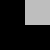
\includegraphics[width=.25in]{../presentation/2x2/Shape1LVL4.png} \\
\tiny{($<$ (y + x) 1), ($<$ (y * x) 1), ($<$ 0 (y + x)), ($<$ 1 (y + x))} & 5 & 
    
\includegraphics[width=.25in]{../presentation/2x2/Shape2LVL5.png}~
    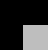
\includegraphics[width=.25in]{../presentation/2x2/Shape1LVL5.png}~
    
\includegraphics[width=.25in]{../presentation/2x2/Shape3LVL5.png}~
    
\includegraphics[width=.25in]{../presentation/2x2/Shape4LVL5.png} \\
\tiny{none} & 6 & empty \\
\tiny{(or ($<$ y  x) ($<$ x  y))} & 7 &
    
\includegraphics[width=.25in]{../presentation/2x2/Shape1LVL7.png}\\
\tiny{(not (or ($<$ y  x) ($<$ x  y)))} & 8 &
    
\includegraphics[width=.25in]{../presentation/2x2/Shape1LVL8.png}
\end{tabular}
\end{center}

\caption{All the 2x2 art with its corresponding complexity.}
\label{fig:2x2}
\end{figure}

From Figure~\ref{fig:2x2}, some things are immediately obvious.  First of all,
as might match one's intuition, the all-black and all-white pictures are the
least complex pictures.  Secondly, one can see that if a formula of size $n$
exists to create a certain picture, then that picture's inverse has a
complexity of one of $n-1$, $n$, or $n+1$.  Examples of this last phenomenon
can be seen between rows 7 and 8, as well as between rows 3 and 4.  This occurs
for the simple reason that adding one symbol ({\tt not}) creates a picture's
inverse.  Also, somewhat intriguingly, we can see gaps at 2 and 6.  Although
there are formulae of size 2, none of those formulae produce a picture that has
not been already produced by formulae of a smaller size.

Seeing all of the pictures, our hypothesis becomes a bit more obvious: What is
the correlation between visual complexity (an inherently subjective notion) and
Kolmogorov complexity?  

\section{Assessing Visual Complexity}

We constructed two websites that asked visitors to choose which of two images
they found to be of greater visual complexity.  One website asked about all the
2x2 art, and the other asked about all of the 3x3 art.  Both such sizes are
small enough to completely enumerate (there are 16 and 512 artworks in each
respective category) as well as small enough to calculate the Kolmogorov
complexity of each artwork.

We then asked users on Twitter as well as local campus students to repeatedly
assess which of two images they found more visually complex.  We treated each
assessment as if it were a competition between two players (artwork one vs
artwork two), and when the user decided upon a winner, we used the TrueSkill
algorithm to update each artwork's relative complexity based on each match's
results.

\section{Results}

% a scatterplot of "measured visual complexity" vs "Kolmogorov complexity"

\section{Summary and Future Work}

We recursively enumerated something that, while R.E., is seldom actually
enumerated, and found the actual Kolmogorov complexity of a large set of very
small artworks.  We then asked a self-selected set of people to assess the
visual complexity of the artworks.  We found a nice relationship between
perceived visual complexity and Kolmogorov complexity, but our results suffer
from ``the law of small numbers''\cite{smallnumbers}.

Anybody interested in reproducing or extending our results is encouraged to
fork our repository on GitHub and use the code however you see fit.  Extending
our results to larger artworks would, in particular, be quite interesting.  
\end{document}



​
